We next evaluate the efficacy of Roots as a performance monitoring and root cause
analysis system for PaaS applications.
To do so, we consider its ability to identify and characterize SLO violations.
For violations that are not caused by a change in workload, we evaluate Roots' ability to identify
the PaaS component that is the cause of the performance anomaly.
Finally, we investigate the performance and scalability of the Roots
prototype. 

%\begin{itemize}
%\item its ability to identify SLO violations,
%\item its ability to characterizes each correctly-identified SLO violation as
%being due to a workload change or a bottleneck,
%\item when there is a bottleneck, its ability to identify the correct
%bottleneck, 
%\item the speed with which it reacts to anomalies, and
%\item its failure rate (accuracy).
%\end{itemize}
%%its ability to detect performance anomalies, and correctly
%%identify the component responsible for each anomaly.  
%Additionally, we wish
%to characterize the overhead introduced by Roots in terms of its effect on
%perceived application performance, and determine the degree to which Roots
%pods enable scalability.

\subsection{SLO Anomaly Detection}

\begin{table}
{\footnotesize
\begin{center}
\begin{tabular}{|c|p{1cm}|p{1cm}|p{1cm}|}
\hline
Faulty Service & $L_1$ (30ms) & $L_2$ (35ms) & $L_3$ (45ms) \\ \hline
datastore & 18 & 11 & 10 \\ \hline
user management & 19 & 15 & 10 \\ \hline
\end{tabular}
\end{center}
}
\vspace{-0.2in}
\caption{\textit{Number of anomalies detected in guestbook app under different SLOs 
($L_1$, $L_2$ and $L_3$) when injecting faults into two different PaaS kernel services.
\label{tab:anomaly_counts}
}}
\vspace{-0.2in}
\end{table}

We first experiment with the SLO-based anomaly detector of Roots
using a simple HTML-producing, Java 
web application called ``guestbook''.
%https://cloud.google.com/appengine/docs/java/gettingstarted/creating-guestbook
This application allows users to login and post comments. It uses the
AppScale  datastore service to persist
posted comments, and the AppScale user management service to handle authentication. 
Each request processed
by guestbook results in two PaaS kernel service
invocations -- one to check if the user is logged in, and 
another to retrieve the existing comments from the datastore. We conduct all
our experiments on a single node AppScale cloud except where specified. The node itself is an Ubuntu
14.04 VM with 4 virtual CPU cores (clocked at 2.4GHz) and 4GB of memory.

We run the SLO-based anomaly detector of Roots on guestbook with a sampling rate of 15 seconds, an analysis
rate of 60 seconds, and a window size of 1 hour. We set the minimum samples count to 100, and
run a series of experiments with different SLOs on the guestbook application. Specifically, we fix
the SLO success probability at 95\%, and set the response time upper bound to $\mu_g + n\sigma_g$. 
$\mu_g$ and $\sigma_g$ represent the mean and standard deviation of the
guestbook's response time. We learn these two parameters \textit{a priori} by benchmarking
the application. Then we obtain three different upper bound values for the guestbook's
response time by setting 
$n$ to 2, 3 and 5 and denote the resulting three SLOs $L_1$, $L_2$ and $L_3$ respectively.

Next, we inject performance faults into the AppScale PaaS by modifying its code
to cause the datastore service to be slow to respond.
This fault injection logic activates once every hour, and
slows down all datastore invocations by 45ms over a period of 3 minutes.
We chose 45ms because it is equal 
to $\mu_g + 5\sigma_g$ for the AppScale deployment under test. 
Therefore this delay is sufficient to violate all three SLOs used in our experiments. 
We also perform experiments in which we inject faults into the user management service of
AppScale. Each experiment is run for a period of 10 hours.

\subsubsection{Anomaly Detection Accuracy}

Table~\ref{tab:anomaly_counts} shows how the number of anomalies detected by 
Roots in a 10 hour period varies when the SLO is changed. The number of anomalies
drops noticeably when the response time upper bound is increased. When the $L_3$
SLO (45ms) is used, the only anomalies detected are the ones
caused by our hourly fault injection mechanism. As the SLO is tightened by lowering the upper bound,
Roots detects additional anomalies. These additional anomalies
result from a combination of injected faults, and other naturally occurring faults
in the system. That is, Roots detects naturally occurring
faults (temporary spikes in application latency), while a number of injected faults
are still in the sliding window of the anomaly detector. Together these two types of
faults caused SLO violations usually several minutes after the fault injection period
has expired.  In each case, however, a manual inspection of the data reveals
that Roots identified \textit{all} of the injected and natural faults correctly,
missing none subject to the tightness of the SLO.

\subsubsection{Anomaly Detection Speed}

\begin{figure}
\centering
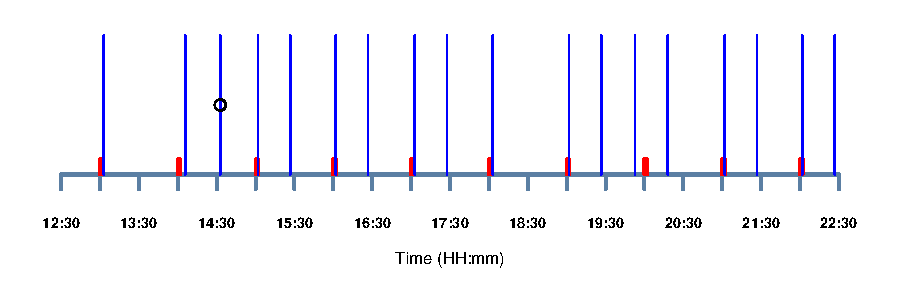
\includegraphics[scale=0.55]{time_line_guestbook_2s}
\vspace{-0.3in}
\caption{\textit{Anomaly detection in guestbook application during a period of 10 hours. 
Red arrows indicate fault injection
at the datastore service. Blue arrows indicate all anomalies detected by
Roots.
}}
\label{fig:time_line_guestbook_2s}
\end{figure}

Next we analyze how fast and often Roots can detect anomalies in an application. We
first consider the performance of guestbook under the $L_1$ SLO while 
injecting faults into the datastore service. Figure~\ref{fig:time_line_guestbook_2s} shows
anomalies detected by Roots as events on a time line. The horizontal axis represents 
passage of time. The red arrows indicate the start of a fault injection period, where each
period lasts up to 3 minutes.
The blue arrows indicate the Roots anomaly detection events.
Note that every fault injection period is immediately followed by an anomaly
detection event, implying near real time reaction from Roots. The only exception is the fault
injection window at 20:00 hours, which is not immediately followed by an anomaly 
detection event. Roots detected another naturally occurring anomaly
(i.e. one
that we did not explicitly inject but nonetheless caused an SLO violation) at 19:52 hours,
which caused the anomaly detector to go into the warm up mode. Therefore Roots
did not immediately react to the faults injected at 20:00 hours. Roots detects the anomaly once it becomes
active again at 20:17. As in the previous
experiment, the detection accuracy is 100\%, as determined by manual
inspection.

%\begin{figure}
%\centering
%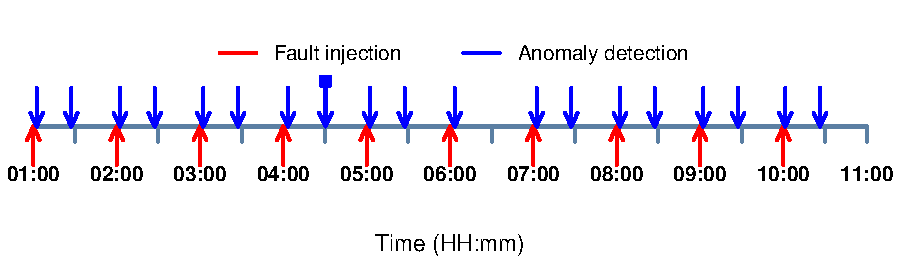
\includegraphics[scale=0.55]{time_line_guestbook_2s_user}
%\caption{Anomaly detection in guestbook application (timeline).}
%\label{fig:time_line_guestbook_2s_user}
%\end{figure}
%
%Figure~\ref{fig:time_line_guestbook_2s_user} shows the anomaly detection time line for the 
%same application and SLO, while faults are being injected into the user management service.
%Here too we see that Roots detects anomalies immediately following each fault injection window.

%\begin{figure}
%\centering
%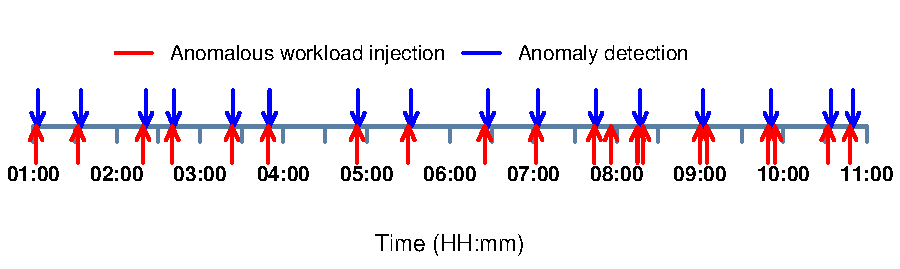
\includegraphics[scale=0.55]{time_line_crud}
%\caption{Path-distribution Anomaly detection in key-value store application (timeline). }
%\label{fig:time_line_crud}
%\end{figure}

%\begin{figure}
%\centering
%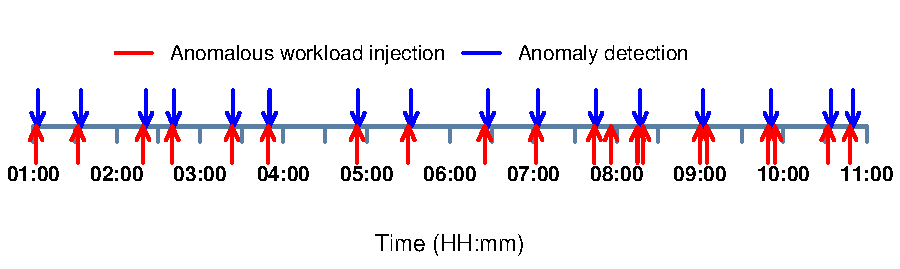
\includegraphics[scale=0.55]{time_line_caching}
%\caption{Anomaly detection in cached key-value store application (timeline).}
%\label{fig:time_line_caching}
%\end{figure}

%\subsection{Path Analyzer Accuracy and Speed}
%
%Next we evaluate the effectiveness and accuracy of the path distribution analyzer. For this we 
%employ a key-value store application. 
%%two different applications.
%%\begin{description}
%%\item[key-value store] 
%This application provides the functionality of an online key-value store.  It allows 
%users to store data objects in the cloud where each object is given a unique key. The objects can then be 
%retrieved, updated or deleted using their keys. Different operations
%(create, retrieve, update and delete) of the application are implemented as separate paths of
%execution in the application source code.
%%\item[cached key-value store] This is a simple extension of the regular key-value store, which adds
%%caching to the read operation using the AppScale's memcache service. The application contains
%%separate paths of execution for cache hits and cache misses.
%%\end{description}
%
%We first deploy the key-value store on AppScale, and populate it with a number of data objects. Then we
%run a test client against it which generates a read-heavy workload. On average this workload
%consists of 90\% read requests and 10\% write requests (create and update). The test client
%is also programmed to randomly send bursts of write-heavy workloads. These bursts consist
%of 90\% write requests on average, and each burst lasts up to 2 minutes. Figure~\ref{fig:time_line_crud}
%shows the write-heavy bursts as events on a time line (indicated by red arrows). Note that almost every burst is
%immediately followed by an anomaly detection event in Roots (indicated by blue arrows). The path
%distribution analyzer detects \textit{every} time the distribution of requests among different paths of execution
%changes significantly. The only time we do not see an anomaly detection event is when multiple
%bursts are clustered together in time (e.g. 3 bursts between 17:04 and 17:24 hours). In this
%case Roots detects the very first burst, and then goes into the warm up mode to collect more data. Therefore
%the bursts that immediately follow do not raise an alarm. These undetected
%events show the conditions under which Roots fails to detect anomalies.
%Events that occur while Roots is gathering a new sample after an anomaly is
%detected are missed.

%In addition,
%Between 20:30 and 21:00 hours we also
%had two instances where the read request proportion dropped from 90\% to 80\% due to random
%chance. This is because our test client randomizes the read request proportion around the 90\% mark. 
%In these two instances the read proportion was deemed too far off from 90\%, and Roots correctly 
%identified them as anomalies.

%We conduct a similar experiment using the cached key-value store. Here, we run a test client that generates a workload
%that is mostly served from the cache. This is done by repeatedly executing read requests on a small
%selected set of object keys. However, the client randomly sends bursts of traffic requesting keys that
%are not likely to be in the application cache, thus resulting in many cache misses. Each burst
%lasts up to 2 minutes. As shown in 
%figure~\ref{fig:time_line_caching}, Roots path distribution analyzer correctly detects the change 
%in the workload (from many cache hits to many cache misses), nearly every time the test client injects a 
%burst of traffic that triggers the cache miss path of the application. The only exception is when
%multiple bursts are clumped together, in which case only the first raises an alarm in Roots.

\subsection{Workload Change Analyzer}

\begin{figure}
\centering
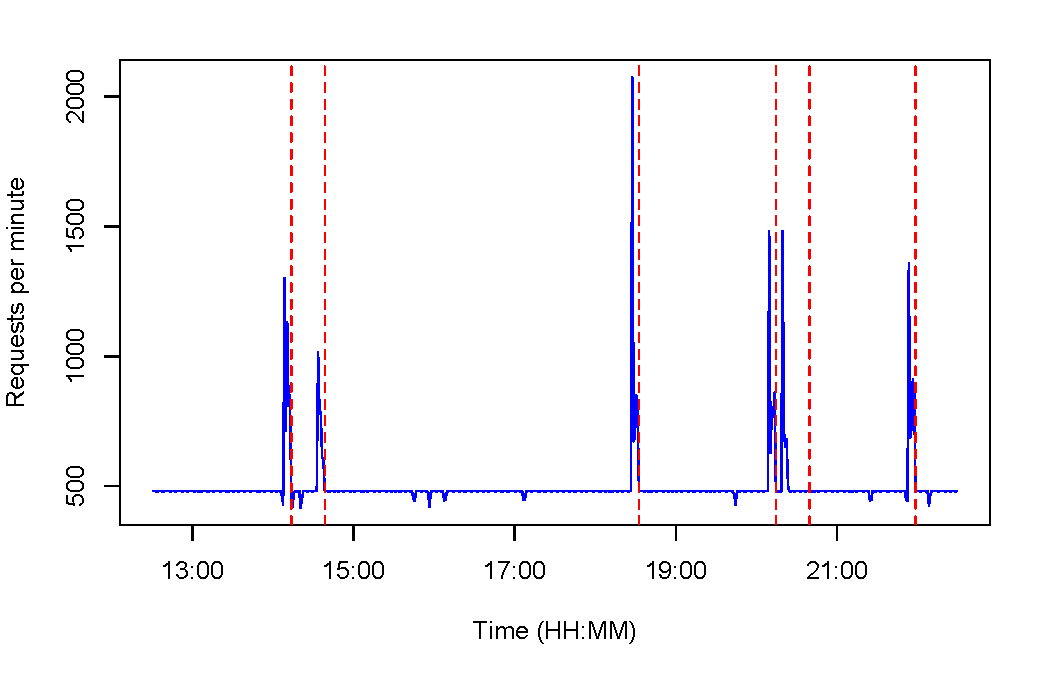
\includegraphics[scale=0.4]{workload_change_trace}
\vspace{-0.2in}
\caption{\textit{Workload size over time for the key-value store application. The test client randomly sends
large bursts of traffic causing the spikes in the plot. Roots anomaly detection events are shown
in red dashed lines.}}
\vspace{-0.2in}
\label{fig:workload_change}
\end{figure}

Next we evaluate the Roots workload change analyzer. In this experiment we run a varying workload
against a test application for 10 hours. The test application is an online key-value store that supports
basic data management operations. The load generating client is programmed
to maintain a mean workload level of 500 requests per minute. However, the client
is also programmed to randomly send large bursts of traffic at times of its choosing. During these bursts 
the client may send more than 1000 requests a minute, thus impacting the performance of
the application server that hosts the key-value store. Figure~\ref{fig:workload_change} shows how
the application workload has changed over time. The workload generator has produced 6 large bursts of traffic during the 
period of the experiment, which appear as tall spikes in the plot.
Note that each burst is immediately followed by a Roots anomaly detection event (shown by red dashed lines). 
In each of these 6 cases, the increase in workload caused a violation of the application performance SLO.
Roots detected the corresponding anomalies, and determined them to be caused by changes in the workload size.
As a result, bottleneck identification was not triggered for any of these anomalies.
Even though the bursts of traffic appear to be momentary
spikes, each burst lasts for 4 to 5 minutes thereby causing a lasting impact on the application performance.
The PELT change point detection method used in this experimental set up is ideally suited for detecting
such lasting changes in the workload level.

\subsection{Bottleneck Identification}

In this subsection, we evaluate the bottleneck identification capability of 
Roots. We first discuss the results obtained using
the guestbook application, and follow with
results obtained using a more complex application.
In the experimental run illustrated in 
figure~\ref{fig:time_line_guestbook_2s}, Roots determined that all the detected anomalies except for one were 
caused by the AppScale datastore service. This is consistent with our expectations since in this experiment we 
artificially inject faults into the datastore. 
The only anomaly that is not traced back to the datastore service is the one that was detected at 14:32 hours.
This is indicated by the blue arrow with a square marker at the top. For this anomaly, Roots concluded that
the bottleneck is the local execution at the application server ($r$). We have verified
this result by manually inspecting the AppScale logs and traces of data collected by Roots. As it turns out,
between 14:19 and
14:22 the application server hosting the guestbook application experienced some problems, which caused
request latency to increase significantly. Therefore we can conclude that Roots has correctly identified 
the root causes of all 18 anomalies in this experimental run
including one that we did not inject explicitly. 

%Similarly, in the experiment shown in figure~\ref{fig:time_line_guestbook_2s_user}, Roots determined
%that all the anomalies are caused by the user management service, except in one instance. This is again
%inline with our expectations since in this experiment we inject faults into the user management service. For the
%anomaly detected at 04:30 hours, Roots determined that local execution time is the primary bottleneck.
%In this case too the server hosting the guestbook application became slow
%during the 04:23 - 04:25 time window, and Roots correctly identified the bottleneck as the local
%application server.

\subsection{A More Complex Example}

\begin{figure}
\centering
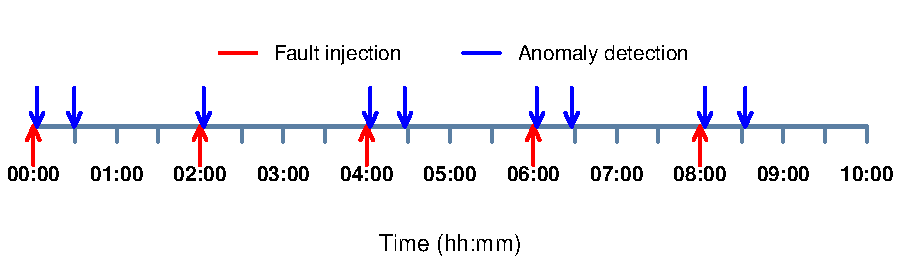
\includegraphics[scale=0.55]{time_line_stocks_1}
\vspace{-0.3in}
\caption{\textit{Anomaly detection in stock-trader application during a period of 10 hours. 
%Red arrows indicate fault injection
%at the 1st datastore query. Blue arrows indicate all anomalies detected by
%Roots during the experimental run.
}}
\vspace{-0.1in}
\label{fig:time_line_stocks_1}
\end{figure}

%\begin{figure}
%\centering
%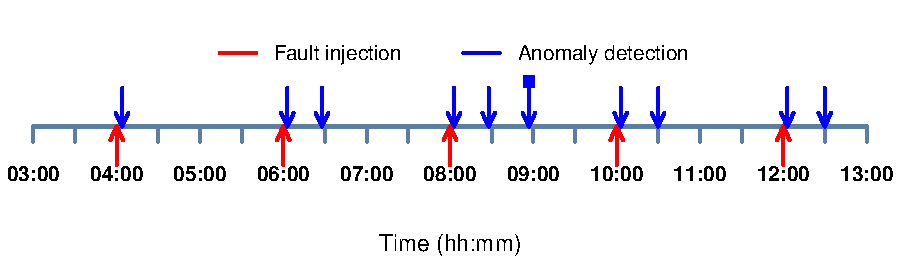
\includegraphics[scale=0.55]{time_line_stocks_2}
%\caption{Anomaly detection in stock-trader application (timeline).}
%\label{fig:time_line_stocks_2}
%\end{figure}

To evaluate how the bottleneck identification performs when an application makes more than 2
PaaS kernel invocations, we conduct another experiment using an application
called ``stock-trader''.
This application allows setting up organizations, and simulating trading of stocks between the
organizations. The two main operations in this application are \textit{buy} and \textit{sell}. Each of
these operations makes 8 calls to the AppScale datastore. 
According to our previous work~\cite{Jayathilaka:2015:RTS:2806777.2806842}, 8 kernel invocations in the
same path of execution is very rare in web applications developed for a PaaS cloud. The probability
of finding an execution path with more than 5 kernel invocations in a sample of PaaS-hosted
applications is less than 1\%. Therefore the stock-trader application is a good extreme case
example to test the Roots bottleneck identification support.
In this experiment we configure the anomaly
detector to check for the response time SLO of 177ms with 95\% success probability.

In one of our experimental runs we inject faults into the first datastore query executed by the buy operation
of stock-trader. The fault injection logic runs every two hours, and lasts for 3 minutes. The duration of
the full experiment is 10 hours. 
Figure~\ref{fig:time_line_stocks_1} shows the resulting event sequence. Note that every fault injection
event is immediately followed by a Roots anomaly detection event. There are also four additional
anomalies in the time line which were SLO violations caused by a combination of injected faults, and
naturally occurring faults in the system. For all the anomalies detected
in this test, Roots correctly selected the first datastore call in the application code as the bottleneck. 
The additional four anomalies occurred because a large number of injected faults were in the sliding window
of the detector. Therefore, it is accurate to attribute those anomalies also to the first datastore query
of the application.

%Figure~\ref{fig:time_line_stocks_2} shows the results from a similar experiment where we inject
%faults into the second datastore query executed by the operation. Here also Roots detects all the
%artificially induced anomalies along with a few extras. All the anomalies, except for one, 
%are determined to be caused by the second
%datastore query of the buy operation. The anomaly detected at 08:56 (marked with a square on top of the blue arrow) 
%is attributed to the fourth datastore query executed by the application. We have manually verified this
%conclusion to be accurate. Since 08:27 (when the previous anomaly was detected), the fourth datastore
%query has frequently taken a long time to execute (again, on
%its own), which resulted in an SLO violation at 08:56 hours.

%In the experiments illustrated in figures~\ref{fig:time_line_guestbook_2s}, 
%\ref{fig:time_line_guestbook_2s_user}, 
%and \ref{fig:time_line_stocks_1} 
%and \ref{fig:time_line_stocks_2} 
%we maintain
%the application request rate steady throughout the 10 hour periods. Therefore as expected,
%the workload change analyzer of Roots did not detect any significant shifts in the workload level. 
%Consequently, none of the anomalies detected in these 4 experiments were attributed to a workload change.
%The bottleneck identification was therefore triggered for each anomaly, always resulting in a performance diagnosis
%involving an application component.

%\begin{figure}
%\centering
%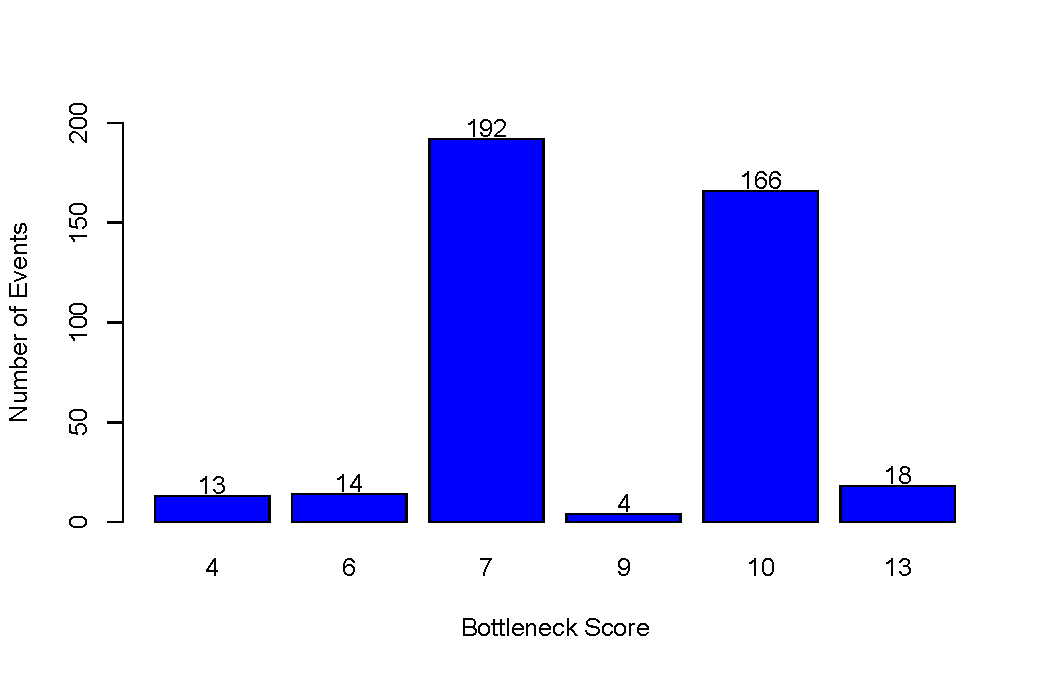
\includegraphics[scale=0.5]{bottleneck_scores}
%\caption{Frequency of different bottleneck scores.}
%\label{fig:bottleneck_scores}
%\end{figure}

%Recall that the bottleneck identification algorithm in Roots
%selects up to four candidate components for each performance anomaly detected, and then ranks them
%by assigning scores to identify the most likely bottleneck. Figure~\ref{fig:bottleneck_scores} shows the breakdown of 407 anomalies
%detected over a period of 3 weeks. X-axis represents the different scores given to candidate components
%by our algorithm. Y-axis shows the number of times a particular score was the highest. 
%According to this result, on 13 occasions Roots determined the bottleneck based on the highest score
%of 4 (score given to the component identified by the relative importance metric). 
%This happens when the algorithm chooses four different candidates
%for the bottleneck. However, this constitutes only 3.2\% of all the anomalies. In 96.8\% of the time Roots saw
%at least two of the four candidates to be the same (score values 6 or higher). This implies that most of the time Roots is able to
%identify bottlenecks with a high level of confidence since two or more candidate detection methods
%agree on their results.

\subsection{Multi-tenant Cluster Setting}

\begin{figure}
\centering
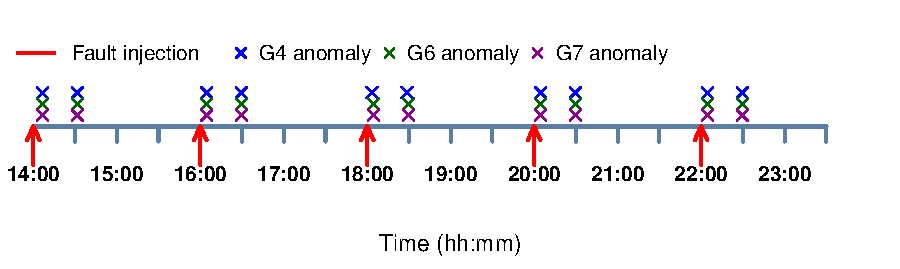
\includegraphics[scale=0.55]{time_line_g1g8}
\vspace{-0.3in}
\caption{\textit{SLO-violation Anomaly detection in 8 applications deployed in
a clustered AppScale cloud.}}
\vspace{-0.2in}
\label{fig:time_line_g1g8}
\end{figure}

To demonstrate how Roots can be used in a multi-node environment, we deploy AppScale
using a cluster of 10 virtual machines (VMs). VMs are provisioned by a
Eucalyptus~\cite{eucalyptus09} (IaaS)
cloud, and each VM is comprised of 2 CPU cores and 2GB memory. Then we proceed
to deploy 8 instances of the guestbook application on AppScale. We use the multi-tenant support
in AppScale to register each instance of guestbook as a different application ($G1$ through $G8$). 
Each application instance has its own datastore namespace, is isolated from the others,
and is accessed via its own public URL. We disable auto-scaling support in 
the AppScale cloud, and inject faults into the datastore service of AppScale by delaying queries from a particular
VM by 100ms.
We identify the VM by its IP address
in our test environment, and shall refer to it as $V_f$ in the discussion. We trigger
the fault injection every 2 hours for a duration of 5 minutes. We then monitor
the applications using Roots for a period of 10 hours. Each anomaly detector is configured
to check for the 75ms response time SLO with 95\% success rate. 
ElasticSearch, Logstash and the Roots pod are deployed on a separate VM. 

Figure~\ref{fig:time_line_g1g8} shows the resulting event sequence. Note that we detect anomalies 
in 3 applications ($G4$, $G6$ and $G7$) immediately after each fault injection. Inspecting the 
topology of our AppScale cluster revealed that these were the only 3 applications that were 
hosted on $V_f$. As a result, bi-hourly fault injection caused their SLOs to
get violated. Other applications did not exhibit any SLO violations since 
the SLO specifies 
a high response time upper bound. In each case Roots detected the SLO violations 2-3 minutes into the fault injection
period. As soon as this happens, the anomaly detectors of $G4$, $G6$ and $G7$ entered their warmup phases.
Our fault injection logic continued to inject faults for at least 2 more minutes. 
Therefore when the anomaly detectors
reactivated after 25 minutes (which is the time to collect the minimum sample count), they each saw another SLO
violation. This is another set of detection events appears in the figure
approximately half an hour after the
original fault injection events.

\subsection{Results Summary}

\begin{table}
{\footnotesize
\begin{center}
\begin{tabular}{|p{2cm}|p{6cm}|}
\hline
Feature & Results Observed in Roots \\ \hline
Detecting accuracy &
The first occurance of all artificially induced anomalies were detected.
Roots also detected several ``natural'' anomalies in AppScale. \\ \hline
Anomaly Differentiation &
All anomalies were correctly identified as either due to workload change or
bottleneck. \\ \hline
Bottleneck Identification &
In all the cases where a bottleneck was identified Roots identified the
correct bottleneck. \\ \hline
Reaction time &
All induced SLO violations were detected as soon
as enough samples of the fault
were taken by the benchmarking process. \\
\hline
\end{tabular}
\end{center}
}
\vspace{-0.2in}
\caption{\textit{Summary of Roots efficacy results.
\label{tab:results_summary}
}}
%\vspace{-0.2in}
\end{table}
Table~\ref{tab:results_summary} summarizes our results.
While not exhaustive, these results indicate that Roots is able to achieve a
high degree of accuracy in detecting and characterizing performance anomalies.
Moreover, for the experimental configurations that we consider, Roots is able to accurately identify
the component that causes each anomaly in a production-quality, open source PaaS.

\subsection{Roots Performance and Scalability}

We evaluate the performance overhead incurred by Roots on the applications deployed in the 
cloud platform. We are particularly interested in understanding the overhead of recording the PaaS kernel
invocations made by each application, since this feature requires some changes to the PaaS kernel
implementation. 
We deploy a number of applications on a vanilla
AppScale cloud (with no Roots), and measure their request latencies. We use
the popular Apache Bench tool to measure the request latency under a
varying number of concurrent clients. We then take the same measurements
on an AppScale cloud with Roots, and compare the results against the ones obtained
from the vanilla AppScale cloud. In both environments we disable the auto-scaling
support of AppScale, so that all client requests are served from a single application
server instance. In our prototype implementation of Roots, the kernel invocation events get buffered in
the application server before they are sent to the Roots data storage. We wish to
explore how this feature performs when the application server is under heavy load.

\begin{table}
{\footnotesize
\begin{center}
\begin{tabular}{|c|p{0.8cm}|p{0.8cm}|p{0.8cm}|p{0.8cm}|}
\hline &
      \multicolumn{2}{c|}{Without Roots} &
      \multicolumn{2}{c|}{With Roots} \\ \hline
    App./Concurrency & Mean (ms) & SD & Mean (ms) & SD\\

\hline
%guestbook/1 & 12 & 3.9 & 12 & 3.7 \\ \hline
guestbook/50 & 375 & 51.4 & 374 & 53.0 \\ \hline
%stock-trader/1 & 151 & 13 & 145 & 13.7 \\ \hline
stock-trader/50 & 3631 & 690.8 & 3552 & 667.7 \\ \hline
%kv store/1 & 7 & 1.5 & 8 & 2.2 \\ \hline
kv store/50 & 169 & 26.7  & 150 & 25.4  \\ \hline
%cached kv store/1 & 3 & 2.8 & 2 & 3.3 \\ \hline
%cached kv store/50 & 101 & 24.8 & 97 & 35.1  \\ \hline
\end{tabular}
\end{center}
}
\vspace{-0.2in}
\caption{\textit{Latency comparison of applications when running on
a vanilla AppScale cloud vs when running on a Roots-enabled
AppScale cloud.}
\label{tab:perf_overhead}
}
%\vspace{-0.2in}
\end{table}

Table~\ref{tab:perf_overhead} shows the comparison of request 
latencies with 50 clients for each of the applications. 
The data shows that Roots does not add a significant overhead
to the request latency in any of the scenarios considered. In all the cases,
the mean request latency when Roots is in use is within or below one standard deviation
from the mean request latency when Roots is not in use.

%The request latency increases when the number of concurrent clients is
%increased from 1 to 50 (since all requests are handled by a single
%application server), but still there is no sign of any detrimental overhead
%from Roots even under load. Since we buffer PaaS kernel invocation
%events in memory, and report them to ElasticSearch asynchronously, and
%out of the request processing flow, there is no measurable impact on
%the request latency from Roots.

%\begin{figure}
%\centering
%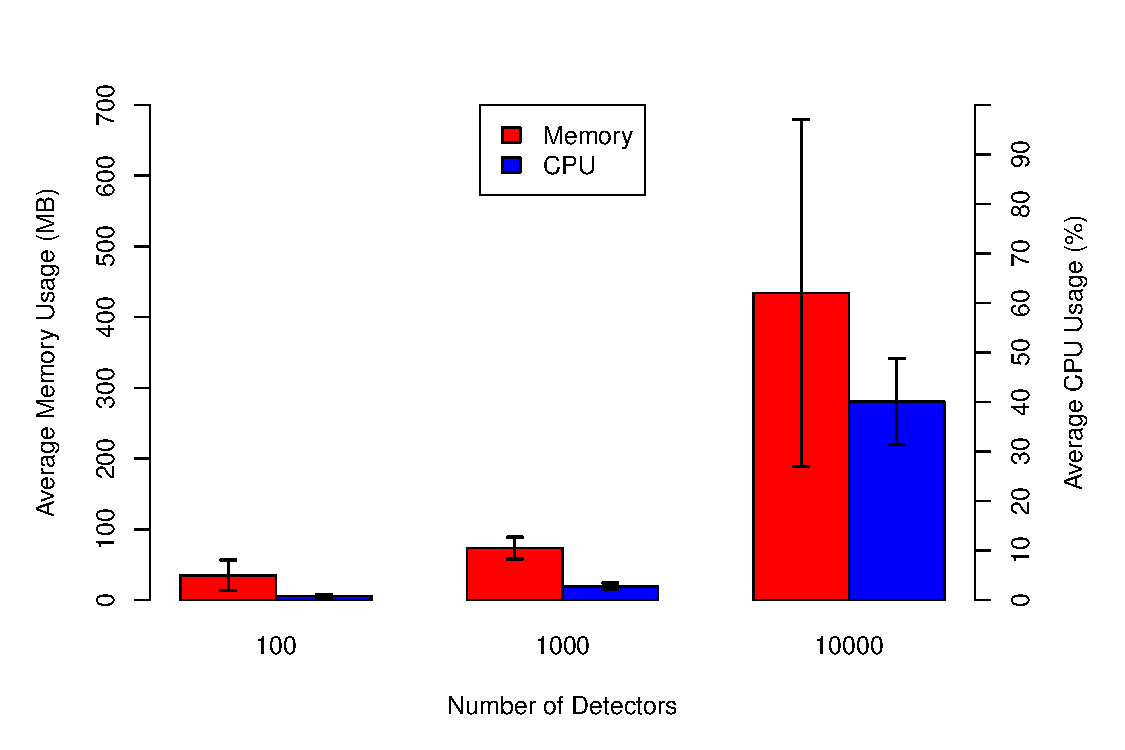
\includegraphics[scale=0.3]{pod_performance}
%\caption{Resource utilization of a Roots pod.}
%\label{fig:pod_performance}
%\end{figure}

Finally, to demonstrate Roots scalability, we deploy
a Roots pod on a virtual machine with 4 CPU cores and 4GB memory.
%
%To simulate monitoring multiple applications, we run multiple concurrent anomaly
%detectors in the pod. Each detector is configured with a 1 hour sliding window.
%We vary the number of concurrent
%detectors between 100 and 10000, and run each configuration for
%2 hours. We track the memory and CPU usage of the
%pod during each of these runs using the jstat and pidstat tools. 
%
%Figure~\ref{fig:pod_performance}
%illustrates the maximum resource utilization of the Roots pod for different counts of
%concurrent anomaly detectors. 
%
With 10000 concurrent detectors, the maximum memory usage of the pod was 778MB and the CPU usage
was 60\% of a single core.  Using just the one machine, with 4 cores and 4GB of
memory, a single pod was able to service 40000 concurrent detectors. 
Since one pod can service a large number of applications simultaneously
 and pods are independent, these results indicate that Roots 
scales in the number of detectors.

%maximum CPU usage is 238\%, where 400\% is the available limit
%for 4 CPU cores. The maximum memory usage in this case is only 778 MB. 
%Since each anomaly detector operates with a fixed-sized window, and they
%bring additional data into memory only when required, the memory
%usage of the Roots pod generally stays low. In particular, the average resource usage
%is far less than the maximum usage values shown in figure~\ref{fig:pod_performance}. 
%For example, in case of 10000 detectors, the average CPU usage is only 32\%, and 
%the average memory usage is 507 MB. We also experimented with larger concurrent
%detector counts, and we were able to pack up to 40000 detectors into the pod before
%getting constrained by the CPU capacity of our quad-core VM.
%This result implies that we can monitor tens of thousands 
%of applications using a single pod, thereby scaling up to a very large number
%of applications using only a handful of pods.
%
